
\section{Adaptation à un cas non stationnaire}
\label{sec:nonstat}

\indent Les résultats présentés dans les sections précédentes se référent à des cas stationnaires, avec les surfaces fixes, mais une situation qu'on veut considérer aussi  est celle où les objets bougent. Dans ce cas, il faut à chaque pas de temps actualiser la fonction Level Set et adapter le maillage autour de la nouvelle position de la surface. La procédure adoptée est la suivante : 

\begin{enumerate}
	\item Pour tout noeud du maillage, calculer la fonction Level Set par rapport à la position actuelle de l'objet, et la fonction \(u\) à adapter (equation \eqref{eq:atan});
	\item Adapter le maillage à la fonction \(u\);
	\item Faire bouger la surface de l'objet (indépendamment de la position des noeuds)
\end{enumerate}

\indent L'objectif de cette procédure est de faire chaque adaptation à partir du dernier maillage adapté, au lieu de partir du maillage non adapté à chaque pas du mouvement. Ainsi, on peut éviter de garder en mémoire toute la structure du maillage de référence et du maillage adapté. Il faut pourtant garder au moins les aires et les vecteurs normaux du maillage, parce que, en raison du modèle adopté, toutes les adaptations doivent utiliser le même maillage de référence.

\indent Les figures \ref{fig:circleLSAdv} et \ref{fig:nacaLSAdv} présentent deux exemples de cette procédure, le premier pour l'advection d'un cercle et le deuxième pour l'oscillation de l'aile Naca. Les mouvements on été discrétisées en 20 pas, et chaque itération a été réalisée avec 20 ou 30 itérations, respectivement.

\indent On peut observer qu'on obtient à chaque pas une bonne adaptation à la position actuelle de la fonction Level Set, mais que les positions précédentes ne sont pas complètement "désadaptées", même que son trace soit faible. En effet, les tests montrent que le passage d'une adaptation à la prochaine se fait de deux manières, soit par le mouvement des points d'une région adaptée à l'autre, soit par le "dérafinement" d'une région. On a observé que le deuxième est plus lente que le premier, et ainsi on aurait besoin d'un plus grand nombre d'itérations. Néanmoins, pour justifier l'application de cette procédure, il faut trouver un équilibre entre le temps d'exécution et la qualité des résultats.

\begingroup
	\begin{minipage}[t]{.5\linewidth}
		\centering
		 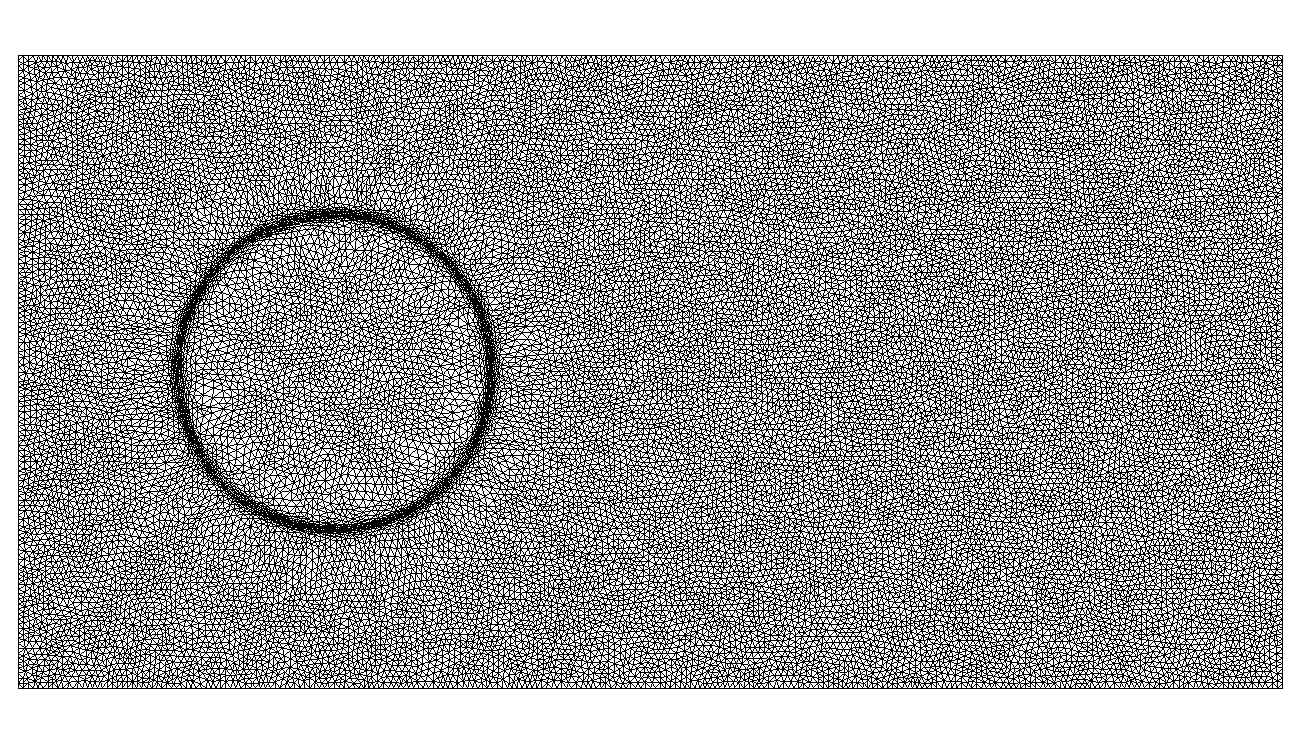
\includegraphics[scale=.15]{Bordeaux/figures/LSAdvection/CircleAdvNew0.png}
		 \captionof{subfigure}{Pas n. 0}
	\end{minipage}
	\begin{minipage}[t]{.5\linewidth}
		\centering
		 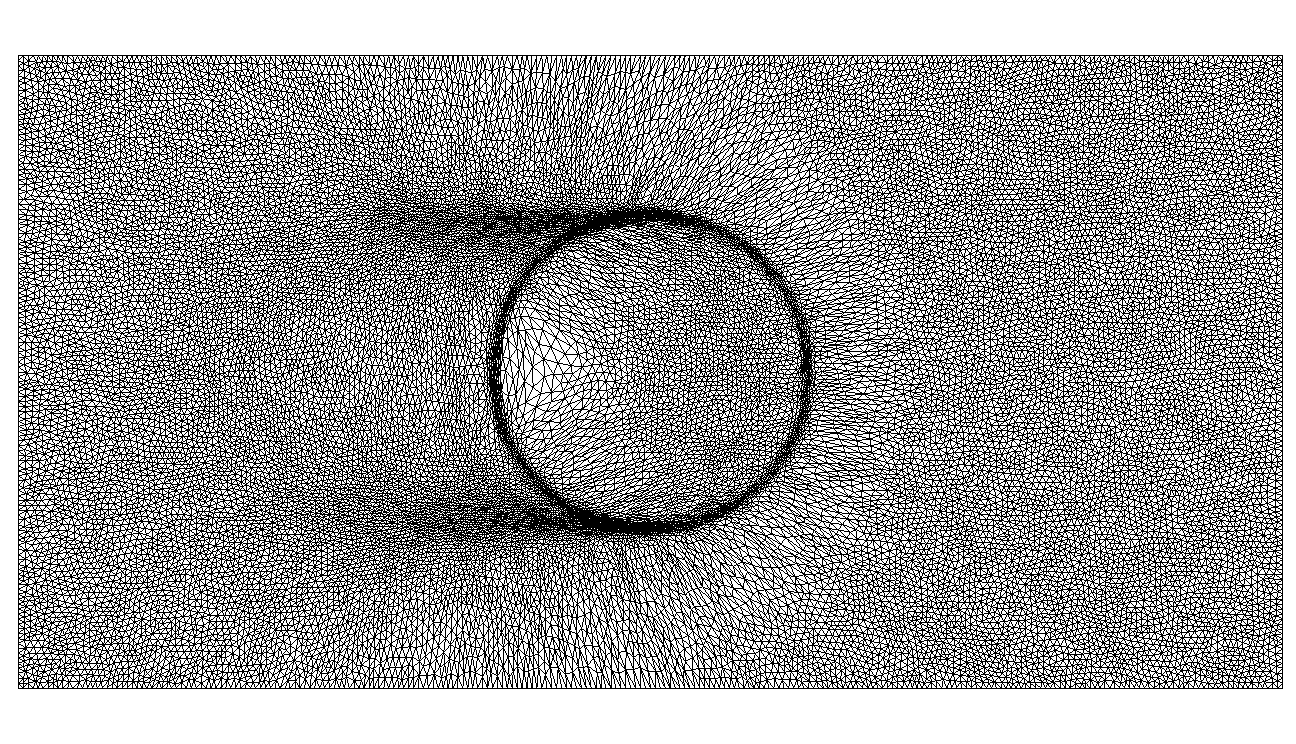
\includegraphics[scale=.15]{Bordeaux/figures/LSAdvection/CircleAdvNew10.png}
		 \captionof{subfigure}{Pas n. 10}
	\end{minipage}
	\begin{minipage}[t]{1.\linewidth}
		\centering
		 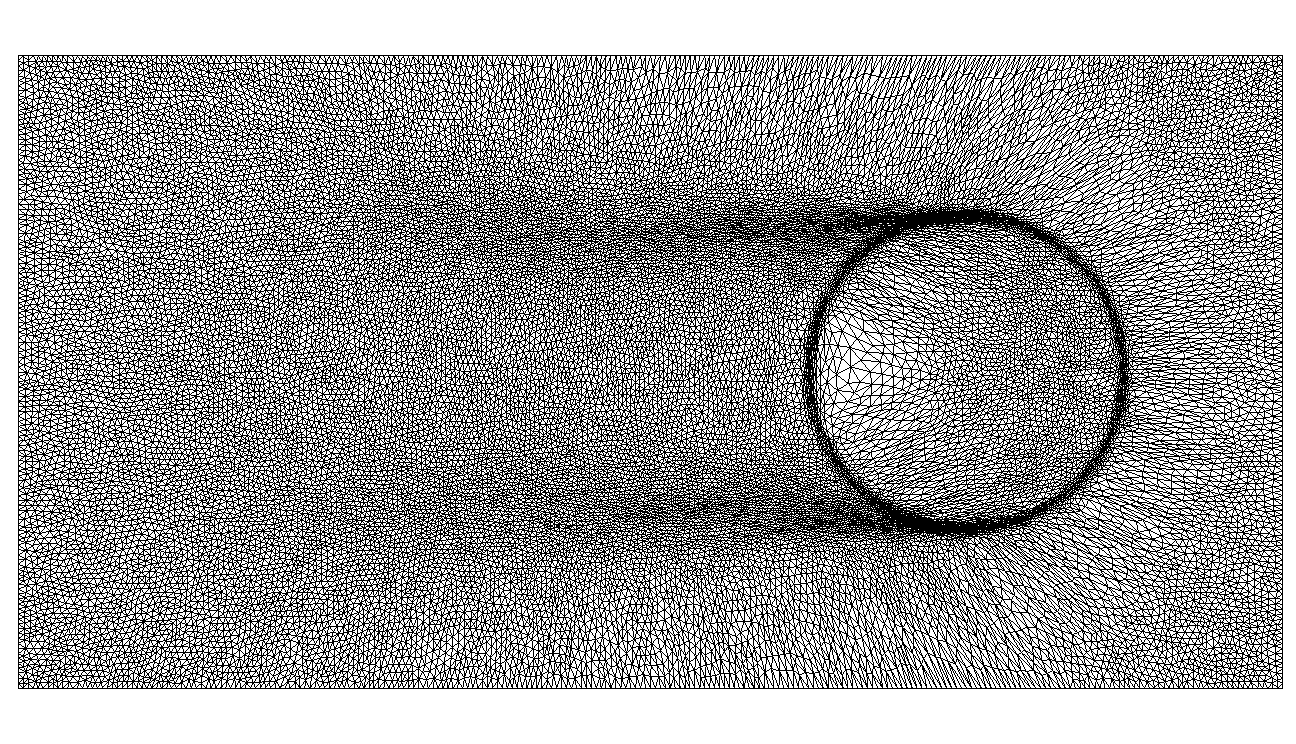
\includegraphics[scale=.15]{Bordeaux/figures/LSAdvection/CircleAdvNew20.png}
		 \captionof{subfigure}{Pas n. 20}
	\end{minipage}
	\captionof{figure}{Advection d'un cercle \label{fig:circleLSAdv}}
\endgroup

\begingroup
	\begin{minipage}[t]{.5\linewidth}
		\centering
		 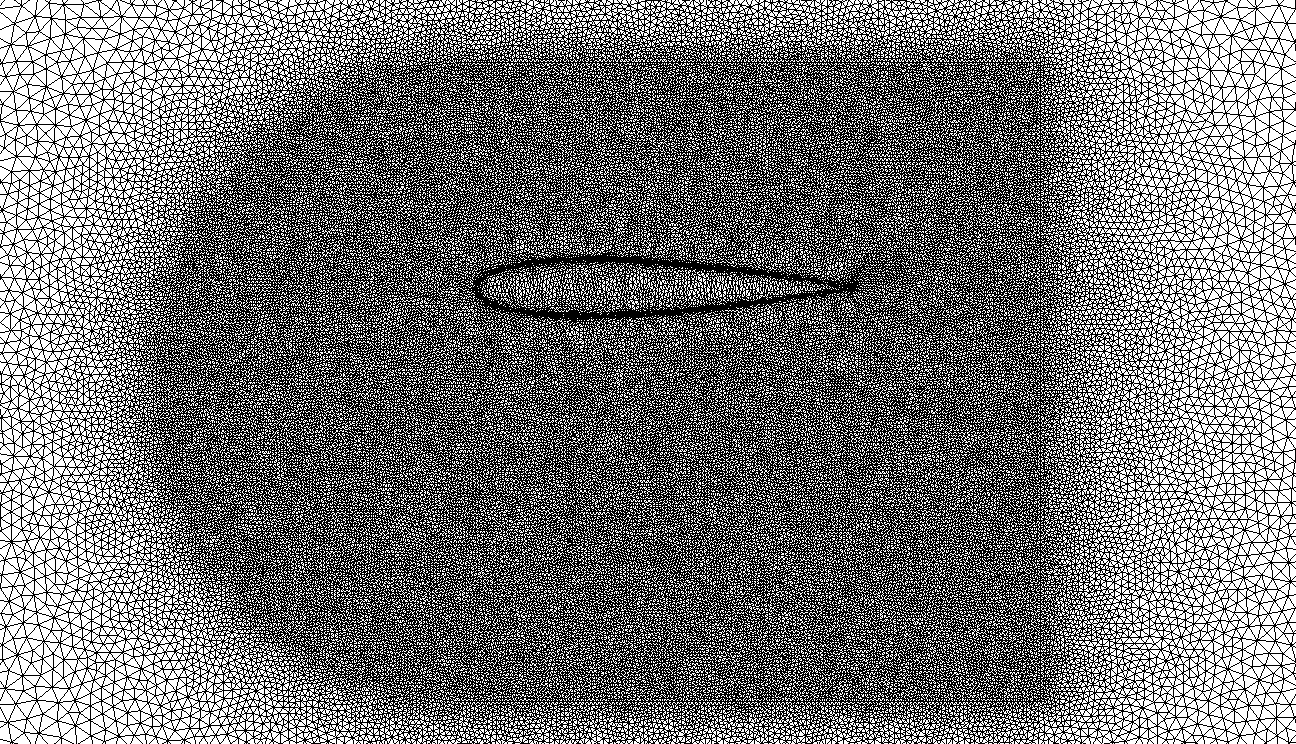
\includegraphics[scale=.15]{Bordeaux/figures/LSAdvection/NacaAdvNew0.png}
		 \captionof{subfigure}{Pas n. 0}
	\end{minipage}
	\begin{minipage}[t]{.5\linewidth}
		\centering
		 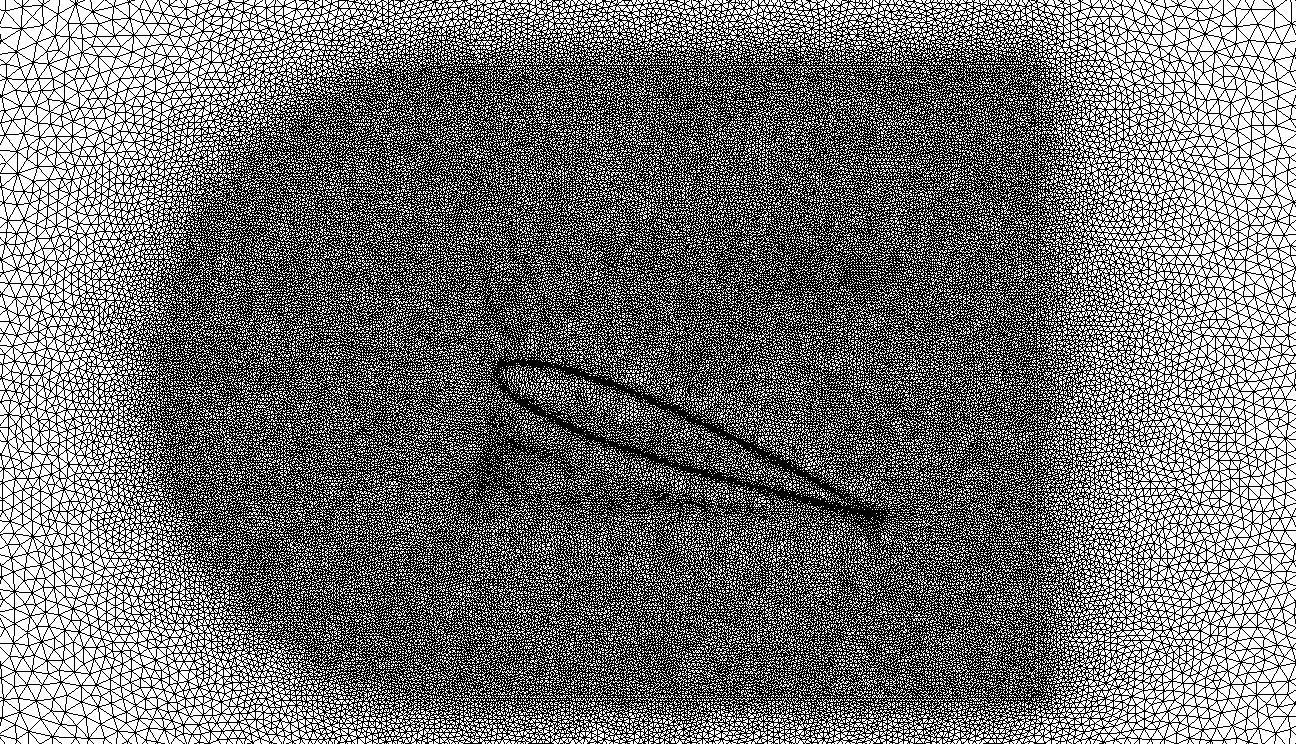
\includegraphics[scale=.15]{Bordeaux/figures/LSAdvection/NacaAdvNew10.png}
		 \captionof{subfigure}{Pas n. 10}
	\end{minipage}
	\begin{minipage}[t]{1.\linewidth}
		\centering
		 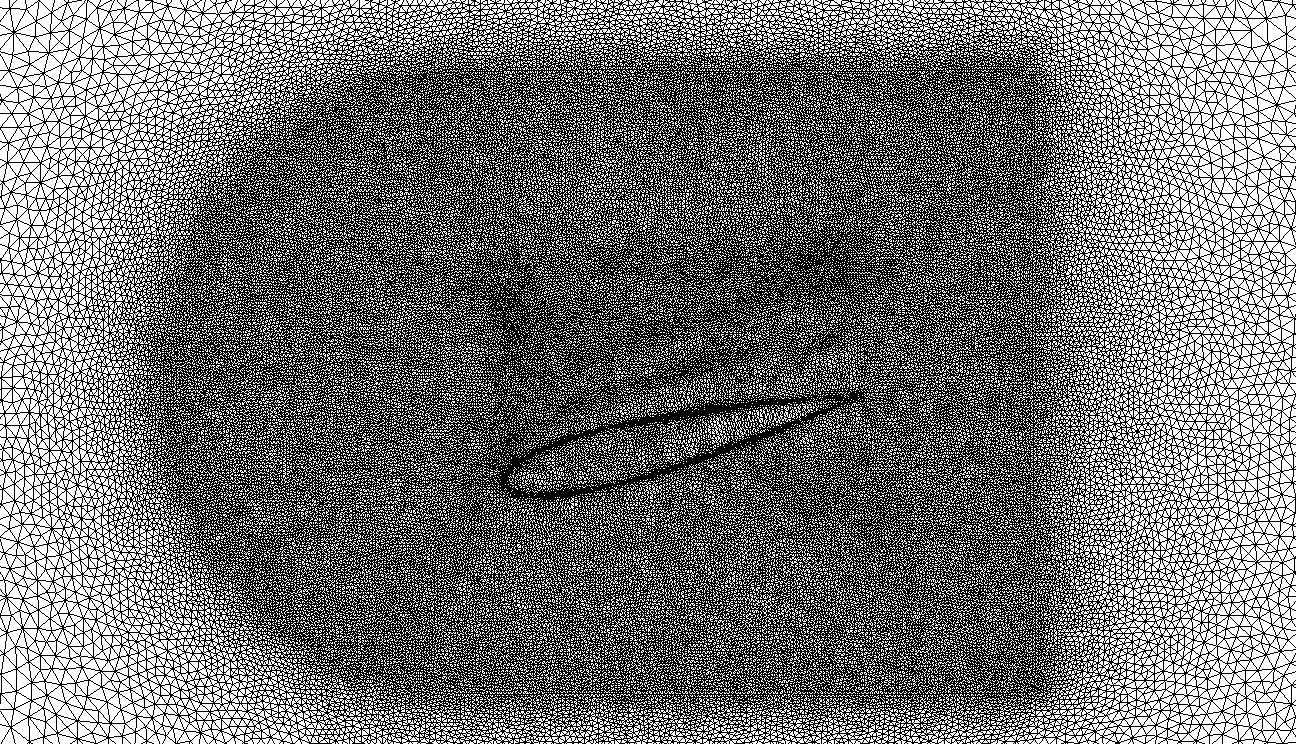
\includegraphics[scale=.15]{Bordeaux/figures/LSAdvection/NacaAdvNew20.png}
		 \captionof{subfigure}{Pas n. 20}
	\end{minipage}
	\captionof{figure}{Naca oscillant \label{fig:nacaLSAdv}}
\endgroup



%\indent L'approche qu'on a d'abord essayé, envisageant une économie de l'espace mémoire utilisé pour l'exécution du programme, était de faire l'adaptation, à chaque pas de temps, à partir du dernier maillage calculé. Néanmoins, les tests ont présenté plusieurs problèmes qui se montrent incontournables avec le modèle d'adaptation qu'on utilise, notamment : 
%
%\begin{itemize}
%	\item Le modèle ne provoque pas un "dé-raffinement" des éléments. Ainsi, dans le résultat final, on peut observer le trace de la marche de l'objet sur le maillage (figure \ref{fig:optim_bad});
%	\item Les éléments raffinés dans un certain pas de temps n'arrivent pas à bouger jusqu'à la nouvelle position, soit en raison de la très fréquente relaxation (principalement quand on discrétise le mouvement de la surface avec un petit pas de temps, car les adaptations successives sont faites presque sur le même endroit), soit parce qu'il sont très éloignés de la nouvelle position (principalement quand le pas de temps est trop grand).
%\end{itemize}
%
%	\begin{figure} [!ht]
%	  \begin{subfigure}{.5\linewidth}
%	    \centering
%	    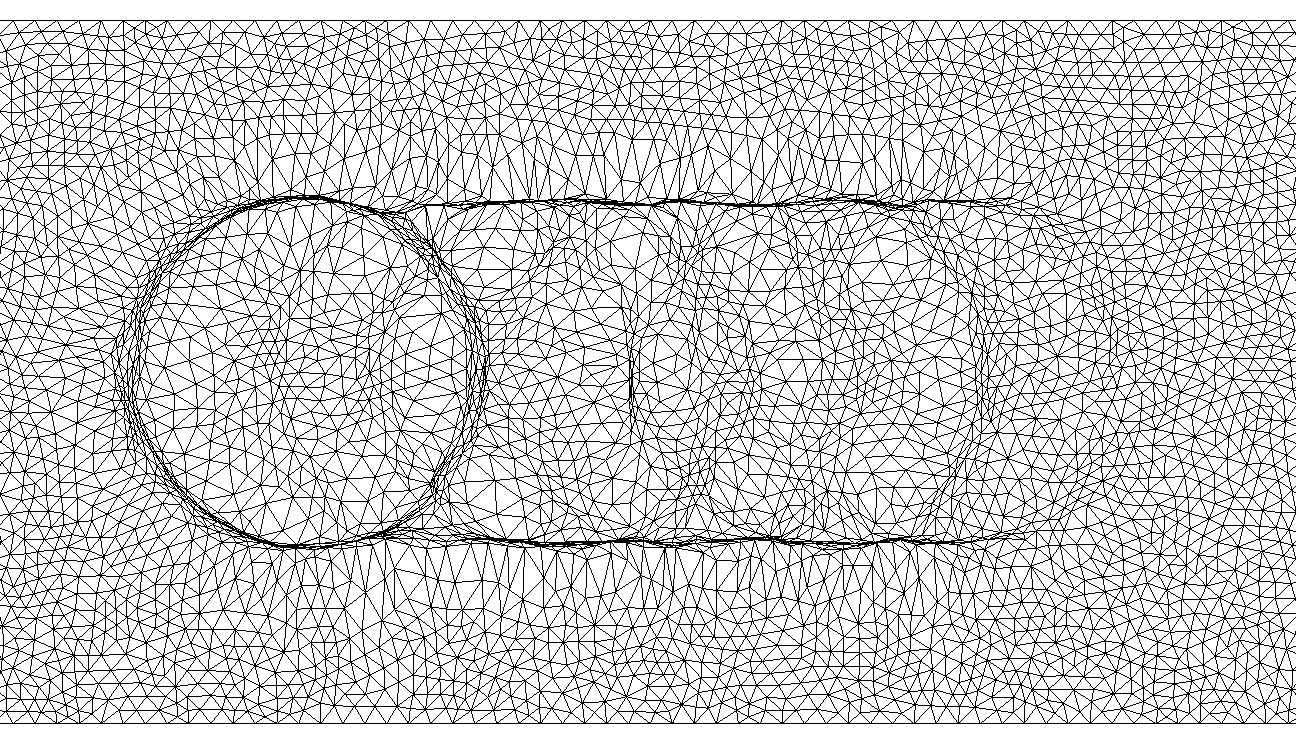
\includegraphics[scale=.12]{figures/optim_bad_circle.png}
%	  \end{subfigure} 
%	  \begin{subfigure}{.5\linewidth}
%	    \centering
%	    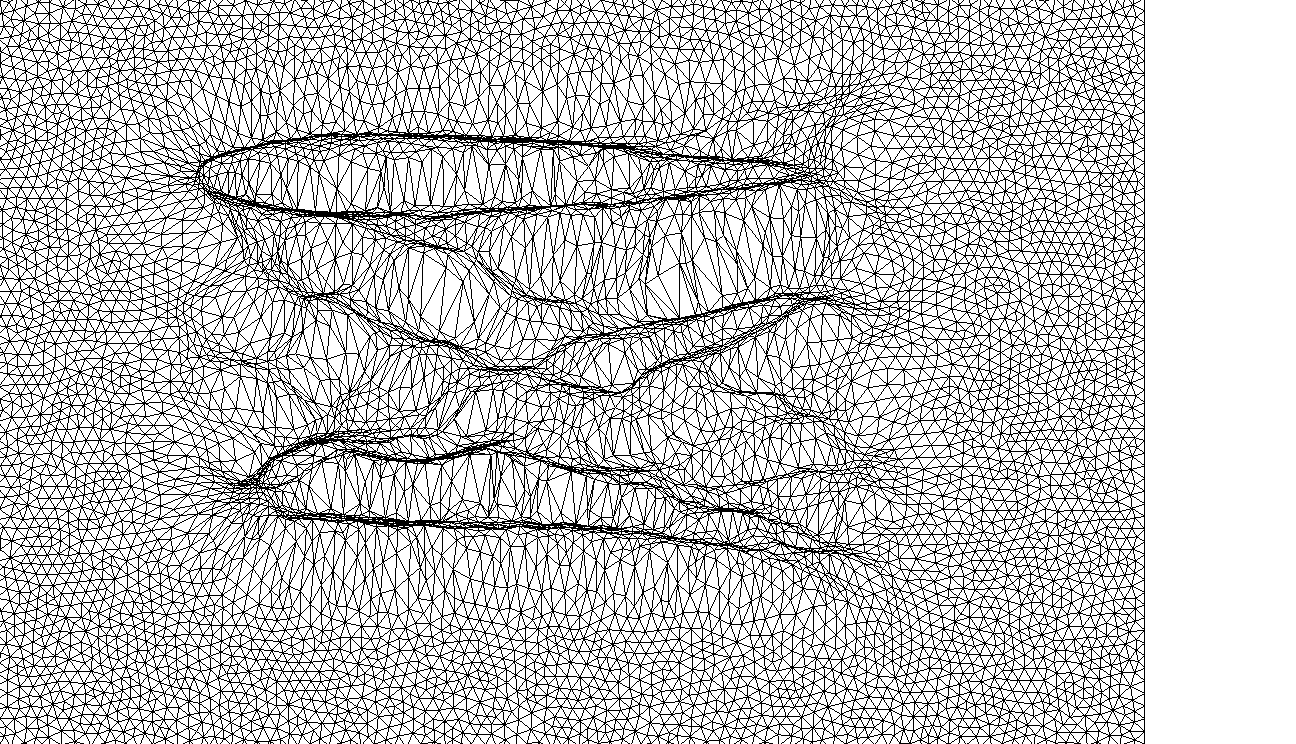
\includegraphics[scale=.12]{figures/optim_bad_naca.png}
%	  \end{subfigure}
%	  \caption{Maillages finaux des adaptions partant du maillage initial à chaque pas du mouvement de la surface \label{fig:optim_bad}}
%	\end{figure}
%
%\indent L'unique solution trouvée, ainsi, est de faire chaque adaptation en partant toujours du maillage initial. On obtient ainsi des très bons résultats, comme montrent les figures \ref{fig:optim_good_1} et \ref{fig:optim_good_2}, car les adaptations sont indépendantes, mais pour cela il faut garder le maillage initial en mémoire.
%
%	\begin{figure} [!ht]
%	  \begin{subfigure}{.5\linewidth}
%	    \centering
%	    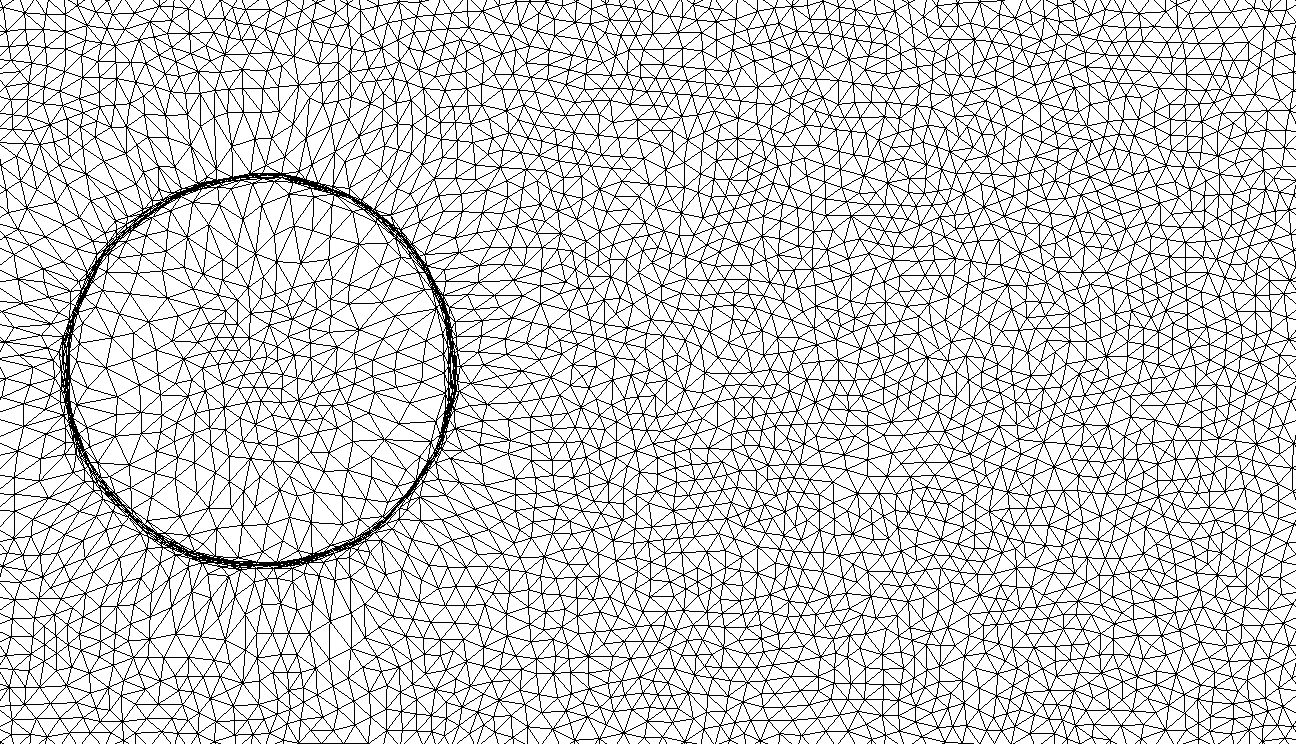
\includegraphics[scale=.12]{figures/optim_good_circle0.png}
%	  \end{subfigure} 
%	  \begin{subfigure}{.5\linewidth}
%	    \centering
%	    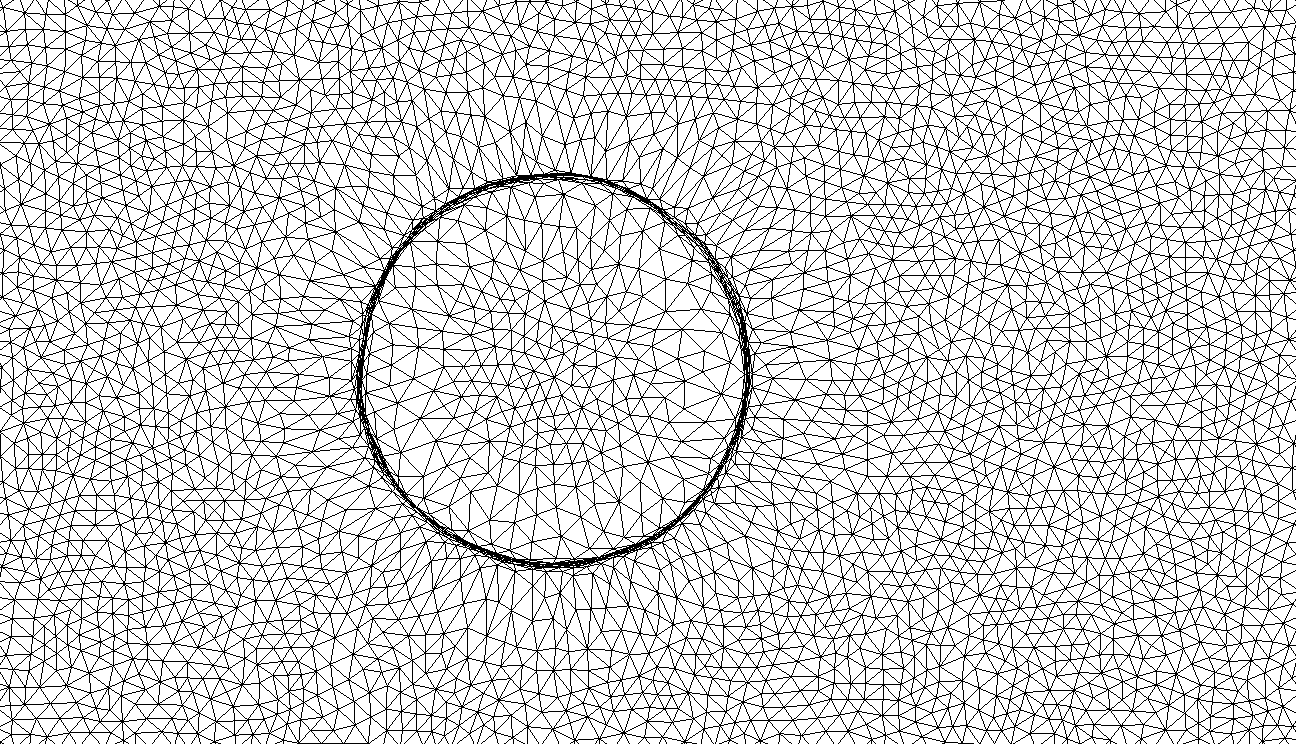
\includegraphics[scale=.12]{figures/optim_good_circle1.png}
%	  \end{subfigure}
%	  \begin{subfigure}{.5\linewidth}
%	    \centering
%	    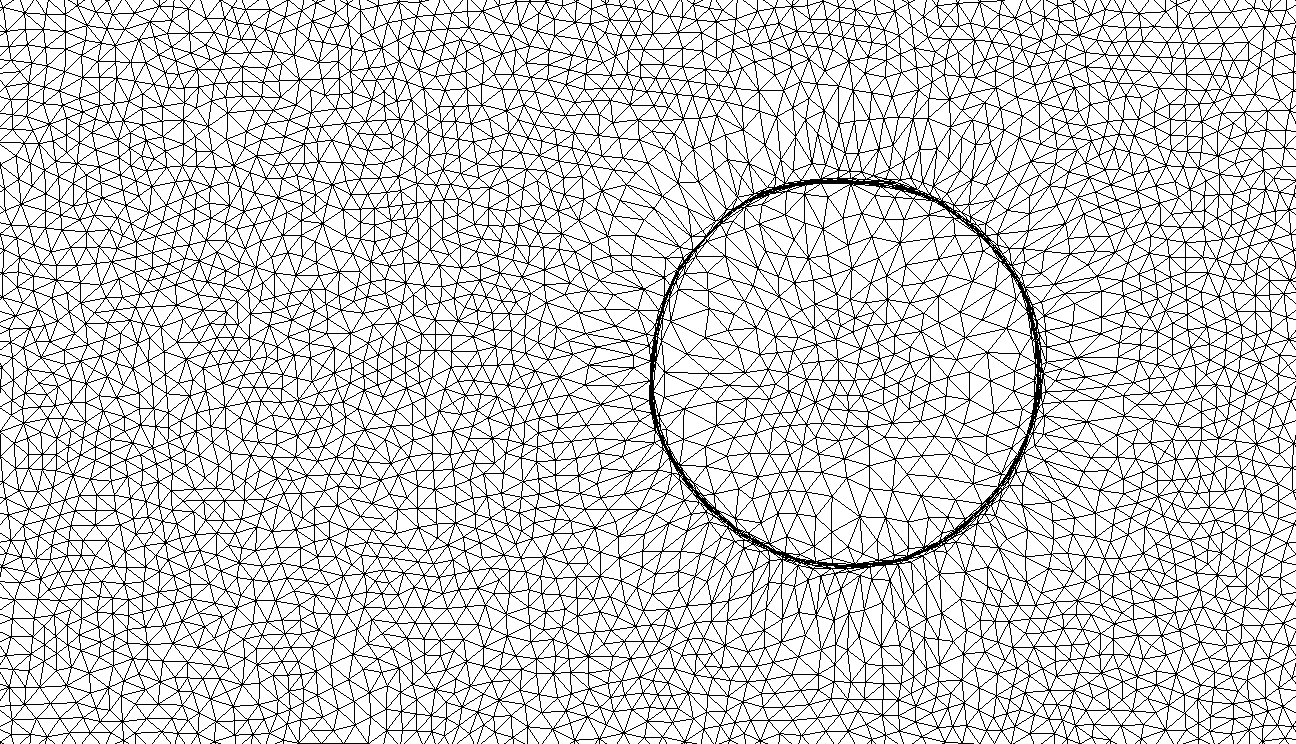
\includegraphics[scale=.12]{figures/optim_good_circle2.png}
%	  \end{subfigure}
%	  \begin{subfigure}{.5\linewidth}
%	    \centering
%	    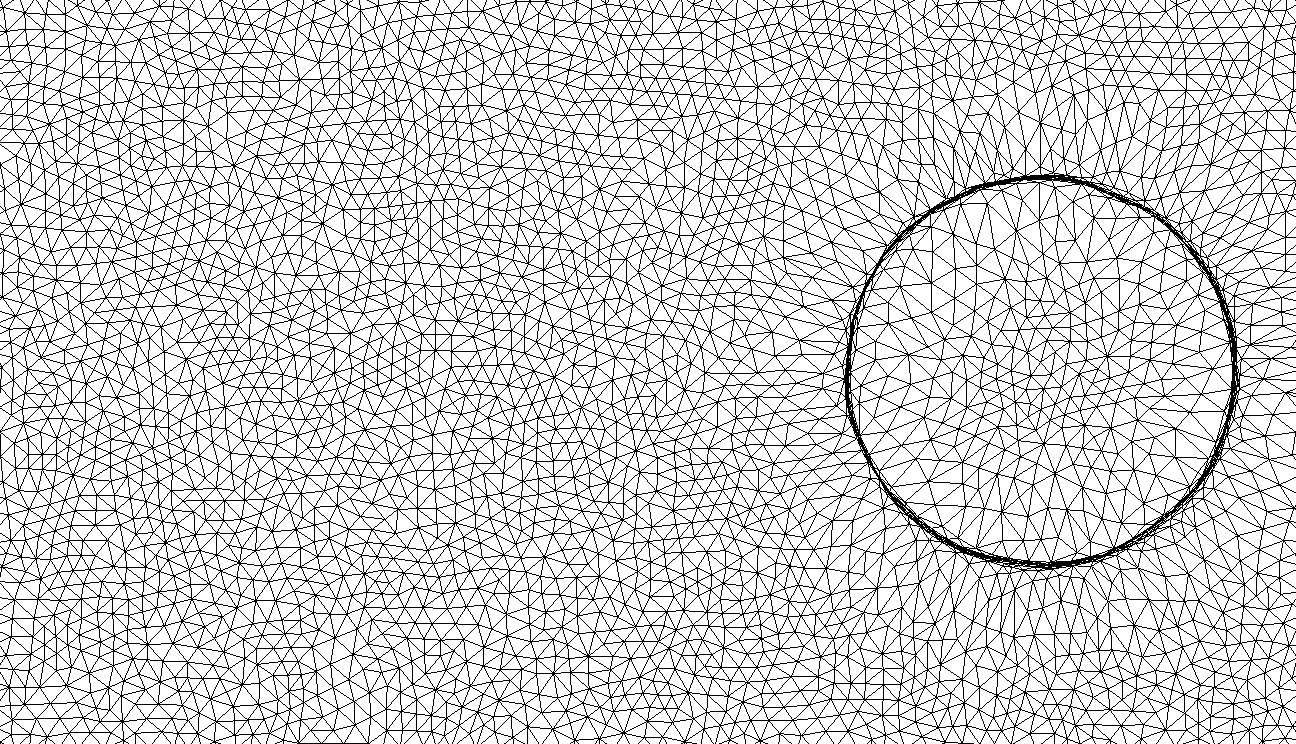
\includegraphics[scale=.12]{figures/optim_good_circle3.png}
%	  \end{subfigure} 
%	  \caption{Adaptation à un cercle advecté \label{fig:optim_good_1}}
%	\end{figure}
%	
%	\begin{figure} [!ht]
%	  \begin{subfigure}{.5\linewidth}
%	    \centering
%	    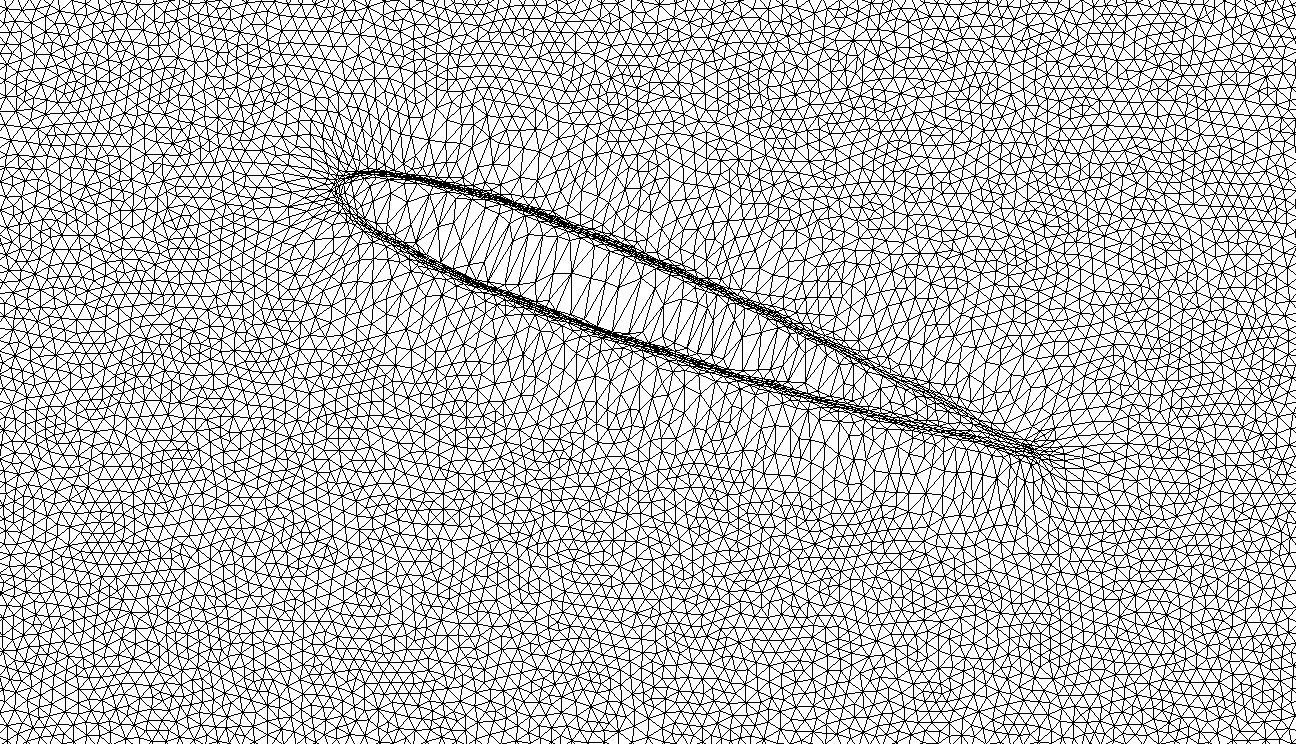
\includegraphics[scale=.12]{figures/optim_good_naca0.png}
%	  \end{subfigure} 
%	  \begin{subfigure}{.5\linewidth}
%	    \centering
%	    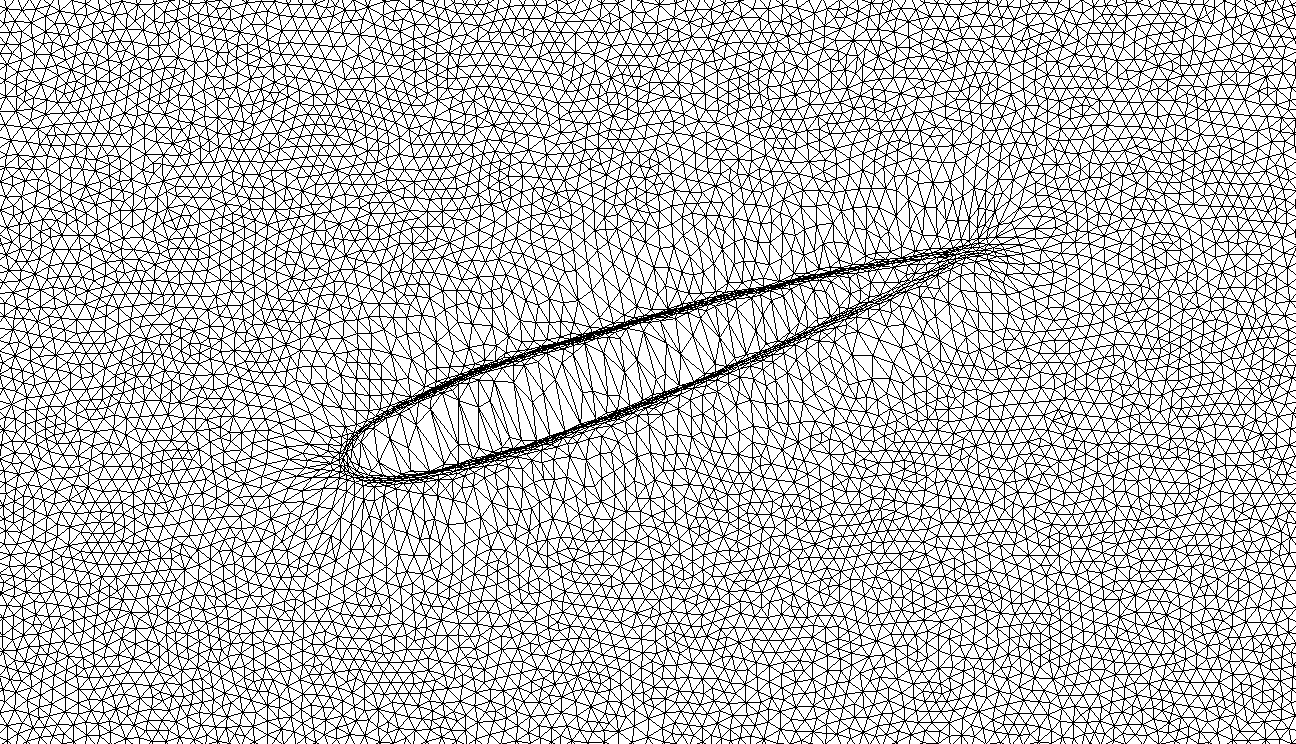
\includegraphics[scale=.12]{figures/optim_good_naca1.png}
%	  \end{subfigure}
%	  \caption{Adaptation au Naca oscillant \label{fig:optim_good_2}}
%	\end{figure}
